\chapter{Discretisation and numerical solution}\label{ch:numerics}

The SEAPODYM underlying partial differential equations (PDE) with initial and boundary conditions eqs.~(\ref{eq:model-1}-\ref{eq:model-3}) are discretised on a regular grid, approximated using the finite-difference method and numerically solved with the alternating-direction implicit (ADI) method \citep{Press}. The numerical approximation scheme and the numerical ADI solver, which are used in SEAPODYM, were developed and implemented by \citet{Sibert-Fournier}  for the general ADR model without an ageing term. It is fully described in \citet{Sibert-Fournier} and \citet{Sibert}. The choice of a classical ADI method despite its known drawbacks, for example, in terms of numerical dispersion, was made for its unconditional stability \citep{Press}, which ensures convergence to a solution for all step sizes and dynamic rates. This method's property enables integration of the numerical model within the optimization method, which implies variations of model parameters. 

The model equations are discretised on a regular Arakawa-A grid. The use of the Arakawa-A grid for the spatial dimensions implies that all quantities are evaluated at the same position, here in the centre of the grid cells. The spatial domain has irregular boundaries. Several boundary conditions are implemented: zero-flux (Neumann) boundary conditions, absorbing (Dirichlet) boundary conditions and conditions for connected east--west borders in the case of a global domain. This chapter describes in detail the discretisation of the model dimensions, the finite-difference approximation of partial derivatives and the numerical solver. 

\section{Discretisation of model dimensions}
\label{sec:discretization}

%\subsection{Discretization of model dimensions}
%\label{sec:dimensions-discretization}

\subsection{Space discretisation}
\label{sec:d-space}

The spatial domain $\Omega\in[X_0,X_m]\times[Y_0,Y_m]$ 
is uniformly discretised in $n_x\times n_y$ cells, 
with a constant step $\Delta x$ (resp. $\Delta y$) along the $x$ (resp. $y$) direction, with the origin $(0,0)$ being the north-west corner of the model domain:

\begin{equation}
  \label{eq:delta-xy}
  \Delta x = (X_m-X_0) / n_x,
  \quad   
  \Delta y = (Y_m-Y_0) / n_y.
\end{equation}
We denote by $(i,j)$, $i=1,\dots n_x$, $j=1,\dots n_y$ the cell that
corresponds to the subdomain 
$[X_0+(i-1)\Delta x,X_0+i\Delta x] \times [Y_0+(j-1)\Delta
  y,Y_0+j\Delta y]$.
All quantities are evaluated at $(x_i,y_j)$, the centre of the cell
$(i,j)$ of the Arakawa-A grid (Figure~\ref{fig:Arakawa-A}), that is
\begin{eqnarray}
  \label{eq:xi}
  x_i &=& X_0+\Big(i-\frac{1}{2}\Big)\Delta x,\quad i=1,\dots, n_x,\\
  \label{eq:yj}
  y_j &=& Y_0+\Big(j-\frac{1}{2}\Big)\Delta y,\quad j=1,\dots, n_y.
\end{eqnarray}


\begin{figure}
   \centering
    \vbox{
    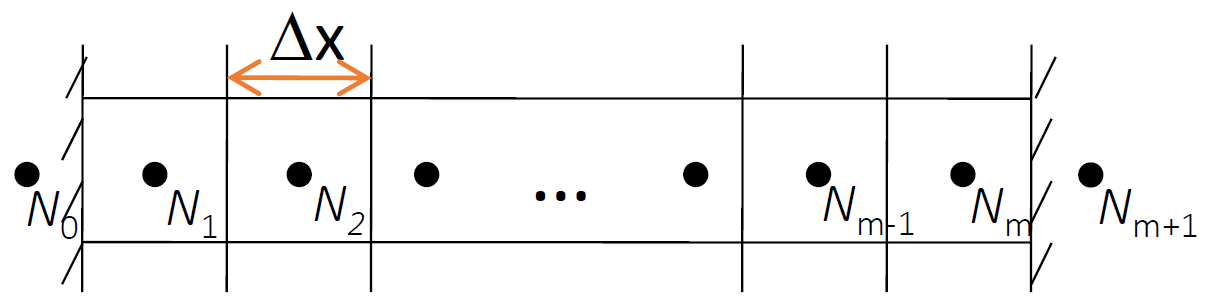
\includegraphics[width=0.5\textwidth]{chapter2/figs/Arakawa-A}
   }
   \caption{Regular Arakawa-A grid used in numerical approximation of SEAPODYM equations. The quantity $N_i=N(x_i,\cdot)$ is the population density described by model eq.~\eqref{eq:model-1}. }
   \label{fig:Arakawa-A}
 \end{figure}

\subsection{Time discretisation}
\label{sec:d-time}

The ADR equation is numerically solved using a multi-incremental algorithm.
The time period $[T_0,T_m]$ is first split into $n_K$ steps or \textbf{outer loops}:
\begin{equation}
  \label{eq:delta-T}
  \Delta T=(T_m-T_0)/n_T,\quad T_K=T_0+K\Delta T,\quad K=0,\dots,n_T.
\end{equation}
where the coefficients of the ADR equation are supposed to be constant. 
Each outer loop is in turn discretised into $n_t$ uniform substeps or \textbf{inner-loops}: 
for a given $K\in\{0,n_T-1\}$ we define
\begin{equation}
  \label{eq:delta-t}
  \Delta t=(T_{K+1}-T_{K})/n_t,\quad t_k=T_{K}+k\Delta t,\quad k=0,\dots,n_t.
\end{equation}
This multi-incremental algorithm is applied with an implicit Euler integration scheme (see below) 
that ensures both stability and good approximation of the solution. 


\subsection{Age discretisation}
\label{sec:d-age}

Population age dimension is discretised into age classes: from the first age class including age $a=0$ to the last age class, including the maximal age $\bar{m}$ of the individuals in the population. In addition, the last age class, also called the $A+$ class, is larger in size than the other age classes. Thus, we define $n_a$ age classes characterized by their age intervals  $[a_p, a_{p+1}]$, $p=0,\dots, n_a$ and the age steps (or age class life period) as follows:
\begin{equation}
  \label{eq:Delta-a}
  \Delta a_p  =a_{p+1} - a_p,\quad p=0,\dots, n_a-1,
\end{equation}
\noindent where the age steps $\Delta a_p = const$ and  $\Delta a_{n_a-1}>\Delta a_p$ for $p=0,\dots, n_a-2$ specify uniformity of all age classes but the last one. Mean age of the age class ${(p)}$ is then given as 
\begin{equation}
  \label{eq:cohort-mean-age}
  \widetilde{a}_{p} = \dfrac{a_{p+1}+a_{p}}{2},\quad p=0,\dots, n_a.
\end{equation}


\begin{table}[!htb]
  \centering
  \begin{tabular}{l|l|l|l|l|l}
    \textbf{Dimension} & \textbf{Variable} & \textbf{Range} & \textbf{Index} & \textbf{Range}  & \textbf{Step}\\
    \hline   \hline                                                                    
    x-coordinate      & $x_i$ & $[X_0,X_m]$      & $i$   & $1,\dots,n_x$ & $\Delta x$ \\\hline
    y-coordinate      & $y_j$ & $[Y_0, Y_m]$     & $j$   & $1,\dots,n_y$ & $\Delta y$ \\\hline
    time (outer loop) & $T_K$ & $[T_0,T_m]$      & $K$   & $0,\dots,n_T$ & $\Delta T$ \\\hline
    time (inner loop) & $t_k$ & $[T_K,T_{K+1}]$  & $k$   & $0,\dots,n_t$ & $\Delta t$ \\\hline
    age               & $a_p$ & $[0,\bar{a}]$    & $p$   & $0,\dots,n_a$ & $\Delta a_p$ \\\hline
    \hline
  \end{tabular}
  \caption{\label{tab:indices}Dimension discretisation indices}
\end{table}

\noindent
\textbf{Notation convention}:
\\
\begin{itemize}
    \item Index names and their meaning are shown in Table \ref{tab:indices}.
    \item For a given quantity $Q$ we define
    \begin{align}
      \label{eq:quantity-grid-tk}
      & Q_{k,p,i,j} = Q(t_k, \widetilde{a}_p, x_i,y_j),&
      \\\nonumber \mbox{and}\\
      \label{eq:quantity-grid-Tk}
      & Q_{K,p,i,j} = Q(T_K, \widetilde{a}_p, x_i,y_j).&
    \end{align}
    \item When there is no loss of clarity we may omit dependence of some variables (or indices). 
\end{itemize}

\section{Approximation of equations and numerical scheme}
\label{sec:equation-discrete-and-numerical-scheme}

The partial derivatives of system (\ref{eq:model-1}-\ref{eq:model-3}) are approximated using centred finite differences. Time integration is performed using a two-step splitting method: advection--diffusion and mortality processes are solved using ADI method along spatial directions: $k\to k+\frac{1}{2}$ for the $x$-direction, $k+\frac{1}{2}\to k+1$ for the $y$-direction. The ageing term is integrated outside of the time integration loop.

During an outer loop period $[T_{K-1},T_{K}]$, we consider that the forcings terms (parameters of advection-diffusion and mortality processes) are constant and equal to their value at $T_{K}$ in order to be consistent with the implicit scheme.

\subsection{Age integration} 
\label{sec:age-integration}

The ageing process is taken into account in between the time integration loops once the solution of the ADR equation is computed over the full time step, that is, between the time steps $[T_{K-1},T_K]$ and $[T_K,T_{K+1}]$ (see also section~\ref{sec:algorithm}). The integration of the ageing term is then done by updating the cohort densities as follows:
\begin{equation}
  \label{eq:aging}
  \left\lbrace
  \begin{array}{lcll}
    N_{K,n_a} &=& N_{K,n_a}+N_{K,n_a-1}&\\
    N_{K,p} &=& N_{K,p-1} &\text{for $p=(n_a-1)\to 1$}
  
  \end{array}
  \right.
\end{equation}


\subsection{Time integration}
\label{sec:two-steps-splitting-method}
%
Time integration from time $T_{K-1}$ to time $T_K$ in the ADI method is done using an iterative \textbf{two-step splitting method along spatial directions}. During these two steps, the ageing process $\partial_a N$ is not taken into account, that is, age class index $p$ is kept constant during time integration.

\paragraph{First half step} \mbox{}\\

\noindent The first implicit half inner-loop time step $k\to k+\frac{1}{2}$ along direction $x$ solves for each inner-loop index $k=0 \dots n_t$:
\begin{align}
  \nonumber
  \dfrac{N_{k+\frac{1}{2}}-N_{k}}{\Delta t/2}
  - \dfrac{\partial}{\partial x}
  \left(
    D_K\dfrac{\partial N_{k+\frac{1}{2}}}{\partial x}
  \right)
  + \dfrac{\partial}{\partial x}
  \left(u_K N_{k+\frac{1}{2}}\right)
  &+ M_{K} N_{k+\frac{1}{2}}
  =\\ \label{eq:2steps-ADI-x}
  &\dfrac{\partial}{\partial y}
  \left(
    D_K\dfrac{\partial N_{k}}{\partial y}
  \right)
  - \dfrac{\partial}{\partial y}
  \left(v_KN_{k}\right).
\end{align}

\paragraph{Second half step} \mbox{}\\
 
\noindent The second implicit  half inner-loop time step $k+\frac{1}{2}\to k+1$ along direction $y$
solves for each inner-loop index $k=0 \dots n_t$:
\begin{align}
  \nonumber
  \dfrac{N_{k+1}-N_{k+\frac{1}{2}}}{\Delta t/2}
  - \dfrac{\partial}{\partial y}
  \left(
    D_K\dfrac{\partial N_{k+1}}{\partial y}
  \right)
  &+ \dfrac{\partial}{\partial y}
  \left(v_KN_{k+1}\right)
  =\\\label{eq:2steps-ADI-y}
  &\dfrac{\partial}{\partial x}
  \left(
    D_K\dfrac{\partial N_{k+\frac{1}{2}}}{\partial x}
  \right)
  - \dfrac{\partial}{\partial x}
  \left(u_KN_{k+\frac{1}{2}}\right)
  - M_{K}N_{k+\frac{1}{2}}.
\end{align}

We then apply discretisation operators \eqref{eq:advection-upwind-x}, \eqref{eq:advection-upwind-y}, \eqref{eq:diffusion-x} and \eqref{eq:diffusion-y} 
depending on the considered cell. For clarity we omit the age class index $p$ in the following paragraphs.

\subsection{Partial derivatives approximation}
\label{sec:ad-derivatives}
\noindent Hereafter we denote by $u$ and $v$ the components of the total velocity 
$\mathbf{v} = \mathbf{v}_c + \mathbf{v}_N$ in eq.~\eqref{eq:model-1}. 

\paragraph{Advection terms}\mbox{} \\

\noindent Derivatives
$\dfrac{\partial}{\partial x}\left( uN \right)$ and 
$\dfrac{\partial}{\partial x}\left( vN \right)$ 
are approximated by centred upwind differencing:
\begin{align}
  \label{eq:advection-upwind-x}
 \left.\dfrac{\partial (uN)}{\partial x}\right|_{i,j} &\approx
 \left\lbrace
   \renewcommand{\arraystretch}{2}
   \begin{array}{lcl}
     \dfrac{1}{\Delta x}(u_{i,j}N_{i,j}-u_{i-1,j}N_{i-1,j}) &
     \mbox{if} & u_{i,j} > 0, \\
     \dfrac{1}{\Delta x}(u_{i+1,j}N_{i+1,j}-u_{i,j}N_{i,j}) &
     \mbox{if} & u_{i,j} < 0, 
   \end{array}
   \right.
   \\
   \label{eq:advection-upwind-y}
   \left.\dfrac{\partial (vN)}{\partial y}\right|_{i,j} &\approx
   \left\lbrace
   \renewcommand{\arraystretch}{2}
   \begin{array}{lcl}
     \dfrac{1}{\Delta y}(v_{i,j}N_{i,j}-v_{i,j-1}N_{i,j-1}) &
     \mbox{if} & v_{i,j} > 0, \\
     \dfrac{1}{\Delta y}(v_{j+1,j}N_{i,j+1}-v_{i,j}N_{i,j}) &
     \mbox{if} & v_{i,j} < 0.
   \end{array}
   \right.
\end{align}

\paragraph{Diffusion terms} \mbox{} \\

\noindent Derivatives
% $ \dfrac{\partial}{\partial x} \left( D\dfrac{\partial N}{\partial x} \right)$ and
% $ \dfrac{\partial}{\partial y} \left( D\dfrac{\partial N}{\partial y} \right)$ 
% are approximated using centered differences on the respective segments $[x_{i-\frac{1}{2}},x_{i+\frac{1}{2}}]$
% and $[y_{j-\frac{1}{2}},y_{j+\frac{1}{2}}]$. The values of $D$ at the boundaries of these segments are approximated by an average 
% (i.e. $D_{i+\frac{1}{2}} \approx (D_{i}+D_{i+1})/2$) \cite{Sibert-1999}: we get:
$\dfrac{\partial}{\partial x} \left( D\dfrac{\partial N}{\partial x} \right)$ and
$ \dfrac{\partial}{\partial y} \left( D\dfrac{\partial N}{\partial y} \right)$ are approximated using centred differences evaluated 
as the mean between the forward finite difference and the backward finite difference of the corresponding terms. We get:
\begin{align}
  %\nonumber
  \left.\dfrac{\partial}{\partial x}\left( D\dfrac{\partial N}{\partial x}\right)\right|_{i,j} 
  &=\left.\dfrac{\partial D}{\partial x}\right|_{i,j} \times \left.\dfrac{\partial N}{\partial x}\right|_{i,j} 
  + D_{i,j}\dfrac{\partial^2 N}{\partial x^2}\\
  &\approx \dfrac{1}{2}\left(
    \dfrac{D_{i+1,j}-D_{i,j}}{\Delta x}\times \dfrac{N_{i+1,j}-N_{i,j}}{\Delta x}\right. \nonumber \\
  &  + \left.\dfrac{D_{i,j}-D_{i-1,j}}{\Delta x}\times \dfrac{N_{i,j}-N_{i-1,j}}{\Delta x}\right) \nonumber\\
  &  + D_{i,j}\times\dfrac{N_{i-1,j}-2N_{i,j}+N_{i+1,j}}{\Delta x^2}\\
%   &\approx\dfrac{1}{\Delta x}\left(
%     D_{i+\frac{1}{2},j} \left.\dfrac{\partial N}{\partial x}\right|_{i+\frac{1}{2},j} -
%     D_{i-\frac{1}{2},j} \left.\dfrac{\partial N}{\partial x}\right|_{i-\frac{1}{2},j}
%    \right)
%    \\
%   &\approx \dfrac{1}{\Delta x}\left(
%       \dfrac{D_{i+1,j}+D_{i,j}}{2}\times\dfrac{N_{i+1,j}-N_{i,j}}{\Delta x}\right.\nonumber \\
%   &-
%       \left.\dfrac{D_{i-1,j}+D_{i,j}}{2}\times\dfrac{N_{i,j}-N_{i-1,j}}{\Delta x}
%     \right)
%     \\
  &\approx
  N_{i-1,j}\dfrac{D_{i,j}+D_{i-1,j}}{2\Delta x^2}
  -N_{i,j}\dfrac{D_{i+1,j}+2D_{i,j}+D_{i-1,j}}{2\Delta x^2} \nonumber\\
  \label{eq:diffusion-x}
  &+  N_{i+1,j}\dfrac{D_{i,j}+D_{i+1,j}}{2\Delta x^2} 
  \\\nonumber\\
  \nonumber
  \left.\dfrac{\partial}{\partial y}\left(
      D\dfrac{\partial N}{\partial y}\right)\right|_{i,j}
  &\approx
  N_{i,j-1}\dfrac{D_{i,j}+D_{i,j-1}}{2\Delta y^2}
  - N_{i,j}\dfrac{D_{i,j+1}+2D_{i,j}+D_{i,j-1}}{2\Delta y^2}
  \\\label{eq:diffusion-y}
  &+ N_{i,j+1}\dfrac{D_{i,j}+D_{i,j+1}}{2\Delta y^2}.
\end{align}


\subsection{Numerical scheme}

For a given grid cell inside the model domain (interior cell), we consider four types of neighbours:
\begin{itemize}
\item ocean cell inside the computation domain,
\item ocean cell outside the computation domain,
\item ocean cell within the East--West overlap zone (in the global domain set-up only),
\item land cell.
\end{itemize}
\vskip 10pt

\noindent Hence, the first three types of interior grid cells are open cells and the last one is the closed boundary cell. Hereafter we provide the model numerical scheme in the interior grid cells; depending whether they are open or closed cells.

\subsubsection{Discretised equations in open grid cells}

In the interior cells surrounded by ocean cells the implicit scheme of eq.~(\ref{eq:2steps-ADI-x}) for the first half time step $k\to k+\frac{1}{2}$ uses spatial terms discretised in the x direction. According to upwind differencing of advection terms, these discrete equations account for the positiveness of $u_{K,i,j}$ and $v_{K,i,j}$:
\begin{itemize}
\item Case $u_{K,i,j}>0$ and $v_{K,i,j}>0$ :
\begin{align}
  \label{eq:2steps-ADI-x-upos-vpos}
  \nonumber
    &N_{k+\frac{1}{2},i-1,j}  \left(
    -\dfrac{u_{K,i-1,j}}{\Delta x}
    -\dfrac{D_{K,i,j}+D_{K,i-1,j}}{2\Delta x^2}
    \right)& \\\nonumber
    &+ N_{k+\frac{1}{2},i,j}  \left(
      \dfrac{2}{\Delta t} 
    +\dfrac{u_{K,i,j}}{\Delta x}
    +\dfrac{D_{K,i+1,j}+2D_{K,i,j}+D_{K,i-1,j}}{2\Delta x^2}
    + M_{K,i,j}    
    \right) \\\nonumber
    & + N_{k+\frac{1}{2},i+1,j} \left(
      -\dfrac{D_{K,i,j}+D_{K,i+1,j}}{2\Delta x^2}
    \right) = \\
    &N_{k,i,j-1}\left(\dfrac{D_{K,i,j}+D_{K,i,j-1}}{2\Delta y^2}+\dfrac{v_{K,i,j-1}}{\Delta y}\right)\\\nonumber
    &+ N_{k,i,j}\left(\dfrac{2}{\Delta t}-\dfrac{v_{K,i,j}}{\Delta y}-\dfrac{D_{K,i,j+1}+2D_{K,i,j}+D_{K,i,j-1}}{2\Delta y^2} \right)
    + N_{k,i,j+1}\left(\dfrac{D_{K,i,j}+D_{K,i,j+1}}{2\Delta y^2}\right)
\end{align}
\item Case $u_{K,i,j}>0$ and $v_{K,i,j}<0$:
\begin{align}
  \label{eq:2steps-ADI-x-upos-vneg}
  \nonumber
    &N_{k+\frac{1}{2},i-1,j}  \left(
    -\dfrac{u_{K,i-1,j}}{\Delta x}
    -\dfrac{D_{K,i,j}+D_{K,i-1,j}}{2\Delta x^2}
    \right)& \\\nonumber
    &+ N_{k+\frac{1}{2},i,j}  \left(
      \dfrac{2}{\Delta t} 
    +\dfrac{u_{K,i,j}}{\Delta x}
    +\dfrac{D_{K,i+1,j}+2D_{K,i,j}+D_{K,i-1,j}}{2\Delta x^2}
    + M_{K,i,j}    
    \right) \\\nonumber
    & + N_{k+\frac{1}{2},i+1,j} \left(
      -\dfrac{D_{K,i,j}+D_{K,i+1,j}}{2\Delta x^2}
    \right) 
    = \\
    \nonumber
    &N_{k,i,j-1}\left(\dfrac{D_{K,i,j}+D_{K,i,j+1}}{2\Delta y^2}\right)
    + N_{k,i,j}\left(\dfrac{2}{\Delta t}+\dfrac{v_{K,i,j}}{\Delta y}-\dfrac{D_{K,i,j+1}+2D_{K,i,j}+D_{K,i,j-1}}{2\Delta y^2} \right)\\
    &+N_{k,i,j+1}\left(\dfrac{D_{K,i,j}+D_{K,i,j+1}}{2\Delta y^2}-\dfrac{v_{K,i,j+1}}{\Delta y}\right)
\end{align}
%
\item Case $u_{K,i,j}<0$ and $v_{K,i,j}>0$:
\begin{align}
  \label{eq:2steps-ADI-x-uneg-vpos}
  \nonumber
    &N_{k+\frac{1}{2},i-1,j}  \left(
      -\dfrac{D_{K,i,j}+D_{K,i-1,j}}{2\Delta x^2}
    \right) \\\nonumber
    &+ N_{k+\frac{1}{2},i,j}  \left(
      \dfrac{2}{\Delta t} 
    -\dfrac{u_{K,i,j}}{\Delta x}
    +\dfrac{D_{K,i+1,j}+2D_{K,i,j}+D_{K,i-1,j}}{2\Delta x^2}
    + M_{K,i,j}    
    \right) \\\nonumber
    &+ N_{k+\frac{1}{2},i+1,j} \left(
      \dfrac{u_{K,i+1,j}}{\Delta x}
      -\dfrac{D_{K,i,j}+D_{K,i+1,j}}{2\Delta x^2}
    \right) 
    = \\
    &N_{k,i,j-1}\left(\dfrac{D_{K,i,j}+D_{K,i,j-1}}{2\Delta y^2}+\dfrac{v_{K,i,j-1}}{\Delta y}\right)\\
    \nonumber
    &+ N_{k,i,j}\left(\dfrac{2}{\Delta t}-\dfrac{v_{K,i,j}}{\Delta y}-\dfrac{D_{K,i,j+1}+2D_{K,i,j}+D_{K,i,j-1}}{2\Delta y^2} \right)
    +N_{k,i,j+1}\left(\dfrac{D_{K,i,j}+D_{K,i,j+1}}{2\Delta y^2}\right)
\end{align}
\item Case $u_{K,i,j}<0$ and $v_{K,i,j}<0$:
\begin{align}
  \label{eq:2steps-ADI-x-uneg-vneg}
  \nonumber
    &N_{k+\frac{1}{2},i-1,j}  \left(
      -\dfrac{D_{K,i,j}+D_{K,i-1,j}}{2\Delta x^2}
    \right) \\\nonumber
    &+ N_{k+\frac{1}{2},i,j}  \left(
      \dfrac{2}{\Delta t} 
    -\dfrac{u_{K,i,j}}{\Delta x}
    +\dfrac{D_{K,i+1,j}+2D_{K,i,j}+D_{K,i-1,j}}{2\Delta x^2}
    + M_{K,i,j}    
    \right) \\\nonumber
    &+ N_{k+\frac{1}{2},i+1,j} \left(
      +\dfrac{u_{K,i+1,j}}{\Delta x}
      -\dfrac{D_{K,i,j}+D_{K,i+1,j}}{2\Delta x^2}
    \right) 
    = \\
    \nonumber
    &N_{k,i,j-1}\left(\dfrac{D_{K,i,j}+D_{K,i,j+1}}{2\Delta y^2}\right)
    + N_{k,i,j}\left(\dfrac{2}{\Delta t}+\dfrac{v_{K,i,j}}{\Delta y}-\dfrac{D_{K,i,j+1}+2D_{K,i,j}+D_{K,i,j-1}}{2\Delta y^2} \right)\\
    &+N_{k,i,j+1}\left(\dfrac{D_{K,i,j}+D_{K,i,j+1}}{2\Delta y^2}-\dfrac{v_{K,i,j+1}}{\Delta y}\right).
\end{align}
\end{itemize}

For the second half time step $k+\frac{1}{2} \to k $, the implicit scheme of eq.~(\ref{eq:2steps-ADI-y}) uses spatial derivatives approximated along the $y$ direction and accounts for the positiveness of $u_{K,i,j}$
and $v_{K,i,j}$
\begin{itemize}
\item Case $v_{K,i,j}>0$ and $u_{K,i,j}>0$:
\begin{align}
  \label{eq:2steps-ADI-y-vpos-upos}
  \nonumber
  &N_{k+1,i,j-1}  \left(
    -\dfrac{v_{K,i,j-1}}{\Delta y}
    -\dfrac{D_{K,i,j}+D_{K,i,j-1}}{2\Delta y^2}
  \right) 
  \\\nonumber
  &+ N_{k+1,i,j}  \left(
    \dfrac{2}{\Delta t} 
    +\dfrac{v_{K,i,j}}{\Delta y}
    +\dfrac{D_{K,i,j+1}+2D_{K,i,j}+D_{K,i,j-1}}{2\Delta y^2}\right) 
  \\\nonumber
  & + N_{k+1,i,j+1} \left(
    -\dfrac{D_{K,i,j}+D_{K,i+1,j}}{2\Delta y^2}
  \right) = 
  \\
  \nonumber
  &N_{k+\frac{1}{2},i-1,j}\left(\dfrac{D_{K,i,j}+D_{K,i-1,j}}{2\Delta x^2}
    +\dfrac{u_{K,i-1,j}}{\Delta x}\right)
  \\\nonumber
  &+ N_{k+\frac{1}{2},i,j}\left(\dfrac{2}{\Delta t}-\dfrac{u_{K,i,j}}{\Delta x}
    -\dfrac{D_{K,i+1,j}+2D_{K,i,j}+D_{K,i-1,j}}{2\Delta x^2}- M_{K,i,j} \right)\\
  &+N_{k+\frac{1}{2},i+1,j}\left(\dfrac{D_{K,i,j}+D_{K,i+1,j}}{2\Delta x^2}\right)
\end{align}
\item Case $v_{K,i,j}>0$ and $u_{K,i,j}<0$:
 \begin{align}
   \label{eq:2steps-ADI-y-vpos-uneg}
    \nonumber
  &N_{k+1,i,j-1}  \left(
    -\dfrac{v_{K,i,j-1}}{\Delta y}
    -\dfrac{D_{K,i,j}+D_{K,i,j-1}}{2\Delta y^2}
  \right) 
  \\\nonumber
  &+ N_{k+1,i,j}  \left(
    \dfrac{2}{\Delta t} 
    +\dfrac{v_{K,i,j}}{\Delta y}
    +\dfrac{D_{K,i,j+1}+2D_{K,i,j}+D_{K,i,j-1}}{2\Delta y^2}\right) 
  \\\nonumber
  & + N_{k+1,i,j+1} \left(
    -\dfrac{D_{K,i,j}+D_{K,i+1,j}}{2\Delta y^2}
  \right) = 
  \\
  \nonumber
  &N_{k+\frac{1}{2},i-1,j}\left(\dfrac{D_{K,i,j}+D_{K,i-1,j}}{2\Delta x^2}\right)
  \\\nonumber
  &+ N_{k+\frac{1}{2},i,j}\left(\dfrac{2}{\Delta t}+\dfrac{u_{K,i,j}}{\Delta x}
    -\dfrac{D_{K,i+1,j}+2D_{K,i,j}+D_{K,i-1,j}}{2\Delta x^2}- M_{K,i,j} \right)\\
  &+N_{k+\frac{1}{2},i+1,j}\left(\dfrac{D_{K,i,j}+D_{K,i+1,j}}{2\Delta x^2}
  -\dfrac{u_{K,i+1,j}}{\Delta x}\right)
 \end{align}
\item Case $v_{K,i,j}<0$ and $u_{K,i,j}>0$:
\begin{align}
  \label{eq:2steps-ADI-y-vneg-upos}
  \nonumber
  &N_{k+1,i,j-1}  \left(
    -\dfrac{D_{K,i,j}+D_{K,i,j-1}}{2\Delta y^2}
  \right) 
  \\\nonumber
  &+ N_{k+1,i,j}  \left(
    \dfrac{2}{\Delta t} 
    -\dfrac{v_{K,i,j}}{\Delta y}
    +\dfrac{D_{K,i,j+1}+2D_{K,i,j}+D_{K,i,j-1}}{2\Delta y^2}\right) 
  \\\nonumber
  & + N_{k+1,i,j+1} \left(
    -\dfrac{D_{K,i,j}+D_{K,i+1,j}}{2\Delta y^2}
    +\dfrac{v_{K,i,j+1}}{\Delta y}
  \right) = 
  \\
  \nonumber
  &N_{k+\frac{1}{2},i-1,j}\left(\dfrac{D_{K,i,j}+D_{K,i-1,j}}{2\Delta x^2}
    +\dfrac{u_{K,i-1,j}}{\Delta x}\right)
  \\\nonumber
  &+ N_{k+\frac{1}{2},i,j}\left(\dfrac{2}{\Delta t}-\dfrac{u_{K,i,j}}{\Delta x}
    -\dfrac{D_{K,i+1,j}+2D_{K,i,j}+D_{K,i-1,j}}{2\Delta x^2}- M_{K,i,j} \right)\\
  &+N_{k+\frac{1}{2},i+1,j}\left(\dfrac{D_{K,i,j}+D_{K,i+1,j}}{2\Delta x^2}\right)
\end{align}
\item Case $v_{K,i,j}<0$ and $u_{K,i,j}<0$:
\begin{align}
  \label{eq:2steps-ADI-y-vneg-uneg}
  \nonumber
  &N_{k+1,i,j-1}  \left(
    -\dfrac{D_{K,i,j}+D_{K,i,j-1}}{2\Delta y^2}
  \right) 
  \\\nonumber
  &+ N_{k+1,i,j}  \left(
    \dfrac{2}{\Delta t} 
    -\dfrac{v_{K,i,j}}{\Delta y}
    +\dfrac{D_{K,i,j+1}+2D_{K,i,j}+D_{K,i,j-1}}{2\Delta y^2}\right) 
  \\\nonumber
  & + N_{k+1,i,j+1} \left(
    -\dfrac{D_{K,i,j}+D_{K,i+1,j}}{2\Delta y^2}
    +\dfrac{v_{K,i,j+1}}{\Delta y}
  \right) = 
  \\
  \nonumber
  &N_{k+\frac{1}{2},i-1,j}\left(\dfrac{D_{K,i,j}+D_{K,i-1,j}}{2\Delta x^2}\right)
  \\\nonumber
  &+ N_{k+\frac{1}{2},i,j}\left(\dfrac{2}{\Delta t}+\dfrac{u_{K,i,j}}{\Delta x}
    -\dfrac{D_{K,i+1,j}+2D_{K,i,j}+D_{K,i-1,j}}{2\Delta x^2}- M_{K,i,j} \right)\\
  &+N_{k+\frac{1}{2},i+1,j}\left(\dfrac{D_{K,i,j}+D_{K,i+1,j}}{2\Delta x^2}
  -\dfrac{u_{K,i+1,j}}{\Delta x}\right)
\end{align}
\end{itemize}

\subsubsection{Discretised equations in closed grid cells}
\label{sec:boundary-conditions}

We now write down the model numerical scheme in closed grid cells, that is, neighbouring with either a land or ocean grid cell assigned as a boundary cell considering three types of boundary conditions: 1) Neumann boundary conditions, 2) Dirichlet boundary conditions, and 3) a special case of Dirichlet boundary conditions in the case of the global domain. 

\paragraph{1) Neumann boundary conditions} \mbox{}\\

\noindent Neumann boundary conditions specify impermeability of domain boundaries. These conditions are applied in the case of closed cells, that is, neighbouring with either land cells or ocean cells, for which impenetrability can be assumed due to natural causes. 

Let's use the case of a \textit{left-closed boundary in the $x$-direction and open boundaries in the $y$-direction} in eq.~\eqref{eq:2steps-ADI-x-upos-vpos}: we have 
$N_{k+\frac{1}{2},i-1,j}= N_{k+\frac{1}{2},i,j}$, $D_{K,i-1,j}=0$ and 
$u_{K,i-1,j}=0$. 
Then if $u_{K,i,j}>0$ and $v_{K,i,j}>0$ we get
\begin{align}
  \label{eq:2steps-ADI-x-upos-vpos+Neumann}
  \nonumber
    &N_{k+\frac{1}{2},i,j}  \left(
      \dfrac{2}{\Delta t} 
    +\dfrac{u_{K,i,j}}{\Delta x}
    +\dfrac{D_{K,i+1,j}+D_{K,i,j}}{2\Delta x^2}
    + M_{K,i,j}    
    \right)
    + N_{k+\frac{1}{2},i+1,j} \left(
      -\dfrac{D_{K,i,j}+D_{K,i+1,j}}{2\Delta x^2}
    \right) 
    = \\
    \nonumber
    &N_{k,i,j-1}\left(\dfrac{D_{K,i,j}+D_{K,i,j-1}}{2\Delta y^2}+\dfrac{v_{K,i,j-1}}{\Delta y}\right)
    + N_{k,i,j}\left(\dfrac{2}{\Delta t}-\dfrac{v_{K,i,j}}{\Delta y}-\dfrac{D_{K,i,j+1}+2D_{K,i,j}+D_{K,i,j-1}}{2\Delta y^2} \right)\\
    &+N_{k,i,j+1}\left(\dfrac{D_{K,i,j}+D_{K,i,j+1}}{2\Delta y^2}\right)
\end{align}
%
Also if $u_{K,i,j}<0$ and $v_{K,i,j}>0$ we get
%
\begin{align}
  \label{eq:2steps-ADI-x-uneg-vpos+Neumann}
  \nonumber
    &N_{k+\frac{1}{2},i,j}  \left(
      \dfrac{2}{\Delta t} 
    +\dfrac{D_{K,i+1,j}+D_{K,i,j}}{2\Delta x^2}
    + M_{K,i,j}    
    \right)
    + N_{k+\frac{1}{2},i+1,j} \left(
      \dfrac{u_{K,i+1,j}}{\Delta x}
      -\dfrac{D_{K,i,j}+D_{K,i+1,j}}{2\Delta x^2}
    \right) 
    = \\
    \nonumber
    &N_{k,i,j-1}\left(\dfrac{D_{K,i,j}+D_{K,i,j-1}}{2\Delta y^2}+\dfrac{v_{K,i,j-1}}{\Delta y}\right)
    + N_{k,i,j}\left(\dfrac{2}{\Delta t}-\dfrac{v_{K,i,j}}{\Delta y}-\dfrac{D_{K,i,j+1}+2D_{K,i,j}+D_{K,i,j-1}}{2\Delta y^2} \right)\\
    &+N_{k,i,j+1}\left(\dfrac{D_{K,i,j}+D_{K,i,j+1}}{2\Delta y^2}\right).
\end{align}

\paragraph{2) Dirichlet boundary conditions} \mbox{}\\

\noindent Dirichlet conditions specify the value that a model variable should take at the boundary. This value can be zero (absorbing boundary) to imply the loss of quantity, or non-zero to account for the incoming quantity  from outside the domain. Dirichlet boundary conditions are applied in the case of a regional domain. 
 
Let us take the case of a \textit{left-open-to-global boundary in the $x$-direction and open boundaries in the $y$-direction} in eq.~\eqref{eq:2steps-ADI-x-upos-vpos}: we have 
%$N_{k+\frac{1}{2},i-1,j}= N^{glo}_{k+\frac{1}{2},i-1,j}$ 
$N_{k+\frac{1}{2},i-1,j} = 0$ 
and the corresponding contribution is part of the second member of the equation. For example, if $u_{K,i,j}>0$ and $v_{K,i,j}>0$ we have
\begin{align}
  \label{eq:2steps-ADI-x-upos-vpos+Dirichlet}
  \nonumber
  &N_{k+\frac{1}{2},i,j}  \left(
    \dfrac{2}{\Delta t} 
    +\dfrac{u_{K,i,j}}{\Delta x}
    +\dfrac{D_{K,i+1,j}+2D_{K,i,j}+D_{K,i-1,j}}{2\Delta x^2}
    + M_{K,i,j}    
    \right) \\ \nonumber
    &+ N_{k+\frac{1}{2},i+1,j} \left(
      -\dfrac{D_{K,i,j}+D_{K,i+1,j}}{2\Delta x^2}
    \right) 
    = \\
    \nonumber
    &N_{k,i,j-1}\left(\dfrac{D_{K,i,j}+D_{K,i,j-1}}{2\Delta y^2}+\dfrac{v_{K,i,j-1}}{\Delta y}\right)
    + N_{k,i,j}\left(\dfrac{2}{\Delta t}-\dfrac{v_{K,i,j}}{\Delta y}-\dfrac{D_{K,i,j+1}+2D_{K,i,j}+D_{K,i,j-1}}{2\Delta y^2} \right)\\
    &+N_{k,i,j+1}\left(\dfrac{D_{K,i,j}+D_{K,i,j+1}}{2\Delta y^2}\right).
    % Comment when N^{glo}=0
    % -N^{glo}_{k+\frac{1}{2},i-1,j}  \left(
    % -\dfrac{u_{K,i-1,j}}{\Delta x}
    % -\dfrac{D_{K,i,j}+D_{K,i-1,j}}{2\Delta x^2}
    % \right)
\end{align}

\paragraph{3) Global domain} \mbox{}\\

\noindent In case of a global domain, namely, the domain covering $360^{\circ}$ in a longitudinal direction, we need to take into account fluxes that come through the western (eastern) boundary from the east (west) of the domain. A special case of \textit{cyclic east--west boundary conditions} is implemented in the SEAPODYM numerical scheme. To make sure that the quantity flows through the open east--west boundaries in the context of the ADI method, we extend the computational domain on both sides along the $x$ (longitudinal) direction to create the buffer zone. The eastern (western) buffer zone is then filled with values from the west (east) of the domain. The size of the buffer zone is defined as large enough to cover the maximal distance of the mass movement during one outer time step $[T_{K-1},T_K]$. The discretised equation is then solved on this extended domain, while at the end of the resolution, we only keep the solution over the non-extended part of the domain.

\section{Tridiagonal matrix system and its resolution} 

\noindent The above numerical scheme eqs.~(\ref{eq:2steps-ADI-x-upos-vpos}--\ref{eq:2steps-ADI-x-upos-vpos+Dirichlet}) can be rewritten in matrix form with the matrices on the left-hand side being tridiagonal. For clarity, we use all dimensional notations here, even though the age index $p$ remains constant within the resolution of linear system. Thus, to get the numerical solution of model~(\ref{eq:model-1}) at a given time step, we solve iteratively (inner loop) two systems of linear equations, and each iteration implies resolution of $n_a\times n_y$ and $n_a\times n_x$ systems of linear equations in a two-step time splitting ADI method. 

Thus, at the first half-step we solve $n_a\times n_y$ linear systems of size $n_x\times n_x$ along the $x$-direction:

\begin{align}
\label{eq:matrix-form-x}
 \mathbf{A}_{K,p,j} \cdot \mathbf{N}_{k+\frac{1}{2},p,j} = \mathbf{g}_{k,p,j}
\end{align}

\noindent and then at the second half-step we solve $n_a\times n_x$ linear systems of size $n_y\times n_y$ along the $y$-direction: 

\begin{align}
\label{eq:matrix-form-y}
 \mathbf{B}_{K,p,i} \cdot \mathbf{N}_{k+1,p,i} = \mathbf{h}_{k+\frac{1}{2},p,i}.
\end{align}   

\noindent Vectors $\mathbf{N}_{k+\frac{1}{2},p,j}=(N_{k+\frac{1}{2},p,1,j},\dots,N_{k+\frac{1}{2},p,n_x,j})^{\text{T}}$ and $\mathbf{N}_{k+1,p,i}=(N_{k+1,p,i,1},\dots,N_{k+1,p,i,n_y})^{\text{T}}$ consist of unknown values of population density along the $x$ and $y$ dimensions respectively. These values are found by solving these linear systems with the help of the forward--backward Gauss elimination (LU decomposition) method. 

The right-hand-side vectors $\mathbf{g}_{k,p,j}=(g_{k,p,1,j},\dots,g_{k,p,n_x,j})^{\text{T}}$ in system~\eqref{eq:matrix-form-x}, and $\mathbf{h}_{k+\frac{1}{2},p,i}=(h_{k+\frac{1}{2},p,i,1},\dots,h_{k+\frac{1}{2},p,i,n_y})^{\text{T}}$ in system~\eqref{eq:matrix-form-y} are constructed either from previous step solution, at $K-1$ (for $k=0$), or from an intermediate solution of the Gauss method, at all $k=1,\dots,n_t$, obtained after each iteration of inner loop of the ADI method. Thus, the elements of vector $\mathbf{g}_{k,p,j}$ are computed for given $a=1,\dots,n_a$ and $j=1,\dots,n_y$ from the coefficients of the matrix $\mathbf{B}$ and density at time $k$ as follows:
\begin{equation}
  \label{eq:second-members-x}
  g_{k,p,i,j} = 
  - d_{K,p,i,j}N_{k,p,i,j-1}
  + \left( \dfrac{4}{\Delta t} - e_{K,p,i,j}\right)N_{k,p,i,j} 
  - f_{k,p,i,j}N_{k,p,i,j+1}.
\end{equation}

\noindent The elements of vector $\mathbf{h}_{k+\frac{1}{2},p,i}$ are computed for given $p=0,\dots,n_a$ and $i=1,\dots,n_x$ from the coefficients of the matrix $\mathbf{A}$ and density at time $k+\frac{1}{2}$ as follows:
\begin{equation}
  \label{eq:second-members-y}
  h_{k+\frac{1}{2},p,i,j} = 
  -a_{K,p,i,j}N_{k+\frac{1}{2},p,i-1,j}
  +\left(\frac{4}{\Delta t}-b_{K,p,i,j}\right)N_{k+\frac{1}{2},p,i,j}
  -c_{K,p,i,j}N_{k+\frac{1}{2},p,i+1,j}.
\end{equation}

\noindent Matrix $\mathbf{A}$ of the linear system~\eqref{eq:matrix-form-x} is defined for all $p=1,\dots,n_a$ and for all $j=1,\dots,n_y$ as follows \citep*[notations of][]{Sibert-Fournier}:
\begin{equation}
  \label{eq:A-matrix}
  \mathbf{A}_{K,p,j}=\left(
    \begin{array}{cccccc}
      b_{K,p,1,j} & c_{K,p,1,j} & 0 & \ldots & 0 & 0\\
      a_{K,p,2,j} & b_{K,p,2,j} & c_{K,p,2,j} & 0 & \ldots & 0\\
      0 & a_{K,p,3,j} & b_{K,p,3,j} & c_{K,p,3,j} & \ldots & 0\\
      \vdots & \ddots & \ddots & \ddots & \ddots & \vdots\\
      0 & \ldots & \ldots & a_{K,p,n_x-1,j} & b_{K,p,n_x-1,j}\ & c_{K,p,n_x-1,j}\\
      0 & \ldots & \ldots & 0 & a_{K,p,n_x,j} & b_{K,p,n_x,j}
    \end{array}
  \right).
\end{equation}

\noindent Matrix $\mathbf{B}$ of the linear system~\eqref{eq:matrix-form-y} is defined for all $p=1,\dots,n_a$, and for all $i=1,\dots,n_x$ as follows:
\begin{equation}
  \label{eq:B-matrix}
  \mathbf{B}_{K,p,i}=\left(
    \begin{array}{cccccc}
      e_{K,p,i,1} & f_{K,p,i,1} & 0 & \ldots & 0 & 0\\
      d_{K,p,i,2} & e_{K,p,i,2} & f_{K,p,i,2} & 0 & \ldots & 0\\
      0 & d_{K,p,i,3} & e_{K,p,i,3} & f_{K,p,i,3} & \ldots & 0\\
      \vdots & \ddots & \ddots & \ddots & \ddots & \vdots\\
      0 & \ldots & \ldots & d_{K,p,i,n_y-1} & e_{K,p,i,n_y-1}\ & f_{K,p,i,n_y}\\
      0 & \ldots & \ldots & 0 & d_{K,p,i,n_y} & e_{K,p,i,n_y}\\
    \end{array}
  \right).
\end{equation}

Below we provide the diagonal coefficients of matrices $\mathbf{A}$ and $\mathbf{B}$ given the type of the boundary conditions. 

\subsection{Diagonal coefficients for Neumann boundary conditions} \mbox{}\\

For a given $p=1,\dots,n_a$ and $j=1,\dots,n_y$, the elements of matrix $\mathbf{A}_{K,p,j}$ are\footnote{Note that the diagonal coefficient of matrix $\mathbf{A}$, $a_{K,p,i,j}$, which is always written with four dimensional indices, should not be confused with age notation $a$, nor with discrete age intervals $a_p$.}
 \begin{align}
   \label{eq:matrix-elements-lowerdiag-x}
   a_{K,p,i,j} &= \left\lbrace
     \renewcommand{\arraystretch}{2.5}
     \begin{array}{lll}
       -\dfrac{u_{K,p,i-1,j}}{\Delta x}
       -\dfrac{D_{K,p,i,j}+D_{K,p,i-1,j}}{2\Delta x^2}
       &\mbox{\minitab{open}{right closed}} & u_{K,p,i,j} > 0 \\
       -\dfrac{D_{K,p,i,j}+D_{K,p,i-1,j}}{2\Delta x^2}
       &\mbox{\minitab{open}{right closed}} & u_{K,p,i,j} < 0\\
       0 & \mbox{\minitab{left closed}{}} & 
     \end{array}
     \right.
     \\
     \label{eq:matrix-elements-diag-x}
     b_{K,p,i,j} &=
     \left\lbrace
     \renewcommand{\arraystretch}{2.5}
     \begin{array}{lll}
       \dfrac{2}{\Delta t} 
       +\dfrac{u_{K,p,i,j}}{\Delta x}
       +\dfrac{D_{K,p,i+1,j}+2D_{K,p,i,j}+D_{K,p,i-1,j}}{2\Delta x^2}\\
       + M_{K,p,i,j}    
       &\mbox{open} 
       & u_{K,p,i,j} > 0 \\
       \dfrac{2}{\Delta t} 
       -\dfrac{u_{K,p,i,j}}{\Delta x}
       +\dfrac{D_{K,p,i+1,j}+2D_{K,p,i,j}+D_{K,p,i-1,j}}{2\Delta x^2}\\
       + M_{K,p,i,j}    
       &\mbox{open} & u_{K,p,i,j} < 0\\
       \dfrac{2}{\Delta t} 
       +\dfrac{D_{K,p,i,j}+D_{K,p,i-1,j}}{2\Delta x^2}
       + M_{K,p,i,j}    
       & \mbox{right closed} & u_{K,p,i,j} > 0\\
       \dfrac{2}{\Delta t} 
       -\dfrac{u_{K,p,i,j}}{\Delta x}
       +\dfrac{D_{K,p,i,j}+D_{K,p,i-1,j}}{2\Delta x^2}
       + M_{K,p,i,j}    
       & \mbox{right closed} & u_{K,p,i,j} < 0\\
         \dfrac{2}{\Delta t} 
         +\dfrac{D_{K,p,i+1,j}+D_{K,p,i,j}}{2\Delta x^2}
         + M_{K,p,i,j}    
       &\mbox{left closed} & u_{K,p,i,j} < 0\\
         \dfrac{2}{\Delta t} 
         + \dfrac{u_{K,p,i,j}}{\Delta x}
         +\dfrac{D_{K,p,i+1,j}+D_{K,p,i,j}}{2\Delta x^2}
         + M_{K,p,i,j}    
       &\mbox{left closed} & u_{K,p,i,j} > 0\\
       \dfrac{2}{\Delta t} + M_{K,p,i,j}
       & \mbox{closed}
     \end{array}
   \right.
   \\
   \label{eq:matrix-elements-upperdiag-x}
   c_{K,p,i,j} &=
     \left\lbrace
     \renewcommand{\arraystretch}{2.5}
     \begin{array}{lll}
        \left(
      -\dfrac{D_{K,p,i,j}+D_{K,p,i+1,j}}{2\Delta x^2}
    \right) 
       &\mbox{\minitab{open}{left closed}} & u_{K,p,i,j} > 0 \\
       \left(
         \dfrac{u_{K,p,i+1,j}}{\Delta x}
         -\dfrac{D_{K,p,i,j}+D_{K,p,i+1,j}}{2\Delta x^2}
       \right) 
       &\mbox{\minitab{open}{left closed}} & u_{K,p,i,j} < 0\\
       0 & \mbox{\minitab{right closed}{}} & 
     \end{array}
   \right.
 \end{align}
For a given $i=1,\dots,n_x$ elements of $\mathbf{B}_{K,p,i}$ are given by
 \begin{align}
   \label{eq:matrix-elements-lowerdiag-y}
   d_{K,p,i,j} &= \left\lbrace
     \renewcommand{\arraystretch}{2.5}
     \begin{array}{lll}
       -\dfrac{v_{K,p,i,j-1}}{\Delta y}
       -\dfrac{D_{K,p,i,j}+D_{K,p,i,j-1}}{2\Delta y^2}
       &\mbox{\minitab{open}{bottom closed}} & v_{K,p,i,j} > 0 \\
       -\dfrac{D_{K,p,i,j}+D_{K,p,i,j-1}}{2\Delta y^2}
       &\mbox{\minitab{open}{bottom closed}} & v_{K,p,i,j} < 0\\
       0 & \mbox{\minitab{top closed}{}} & 
     \end{array}
     \right.
     \\
     \label{eq:matrix-elements-diag-y}
     e_{K,p,i,j} &=
     \left\lbrace
     \renewcommand{\arraystretch}{2.5}
     \begin{array}{lll}
       \dfrac{2}{\Delta t} 
       +\dfrac{v_{K,p,i,j}}{\Delta y}
       +\dfrac{D_{K,p,i,j+1}+2D_{K,p,i,j}+D_{K,p,i,j-1}}{2\Delta y^2}\\
       + M_{K,p,i,j}    
       &\mbox{open} & v_{K,p,i,j} > 0 \\
       \dfrac{2}{\Delta t} 
       -\dfrac{v_{K,p,i,j}}{\Delta y}
       +\dfrac{D_{K,p,i,j+1}+2D_{K,p,i,j}+D_{K,p,i,j-1}}{2\Delta y^2}\\
       + M_{K,p,i,j}    
       &\mbox{open} & v_{K,p,i,j} < 0\\
       \dfrac{2}{\Delta t} 
       +\dfrac{D_{K,p,i,j}+D_{K,p,i,j-1}}{2\Delta y^2}
       + M_{K,p,i,j}    
       & \mbox{bottom closed} & v_{K,p,i,j} > 0\\
       \dfrac{2}{\Delta t} 
       -\dfrac{v_{K,p,i,j}}{\Delta y}
       +\dfrac{D_{K,p,i,j}+D_{K,p,i,j-1}}{2\Delta y^2}
       + M_{K,p,i,j}    
       & \mbox{bottom closed} & v_{K,p,i,j} < 0\\
         \dfrac{2}{\Delta t} 
         +\dfrac{v_{K,p,i,j}}{\Delta y}
         +\dfrac{D_{K,p,i,j+1}+D_{K,p,i,j}}{2\Delta y^2}
         + M_{K,p,i,j}    
       &\mbox{top closed} & v_{K,p,i,j} > 0\\
         \dfrac{2}{\Delta t} 
         +\dfrac{D_{K,p,i,j+1}+D_{K,p,i,j}}{2\Delta y^2}
         + M_{K,p,i,j}    
       &\mbox{top closed} & v_{K,p,i,j} < 0\\
       \dfrac{2}{\Delta t} + M_{K,p,i,j}
       &  \mbox{closed}
     \end{array}
   \right.
   \\
   \label{eq:matrix-elements-upperdiag-y}
   f_{K,p,i,j} &=
     \left\lbrace
     \renewcommand{\arraystretch}{2.5}
     \begin{array}{lll}
        \left(
      -\dfrac{D_{K,p,i,j}+D_{K,p,i,j+1}}{2\Delta y^2}
    \right) 
       &\mbox{\minitab{open}{top closed}} & v_{K,p,i,j} > 0 \\
       \left(
         \dfrac{v_{K,p,i,j+1}}{\Delta y}
         -\dfrac{D_{K,p,i,j}+D_{K,p,i,j+1}}{2\Delta y^2}
       \right) 
       &\mbox{\minitab{open}{top closed}} & v_{K,p,i,j} < 0\\
       0 & \mbox{\minitab{bottom closed}{}} & 
     \end{array}
   \right.
 \end{align}

\subsection{Diagonal coefficients for Dirichlet boundary conditions}

\noindent Let us provide the general formulae for movement rates as well as for diagonal coefficients of tridiagonal matrices of linear system that take into account Dirichlet boundary conditions.

First, we define the following expressions to account for the type of neighbouring grid cell
\begin{align}
  \label{eq:global-flag}
  L^g_{i,j} &= \left\lbrace
    \begin{array}{lll}
      1 &\mbox{if} & \mbox{left open-to-global}\\
      0 & \mbox{else}
    \end{array}
  \right.\\
  R^g_{i,j} &= \left\lbrace
    \begin{array}{lll}
      1 &\mbox{if} & \mbox{right open-to-global}\\
      0 & \mbox{else}
    \end{array}
  \right.
\end{align}
We define the movement rates given the closed boundary
\begin{equation}
  \begin{array}{lcll}
    D_{K,p,i-1,j} &=& -D_{K,p,i,j} 
    & \mbox{left-closed}\\
    D_{K,p,i+1,j} &=& -D_{K,p,i,j} 
    & \mbox{right-closed}\\
    u_{K,p,i-1,j} &=& 0
    & \mbox{left-closed}\\
    u_{K,p,i+1,j} &=& 0
    & \mbox{right-closed}\\
    u_{K,p,i,j} &=&
    \max(u_{K,p,i,j},0)
    & \mbox{left-closed}\\
    u_{K,p,i,j} &=&
    \min(u_{K,p,i,j},0)
    & \mbox{right-closed}
  \end{array}
\end{equation}
We update the expressions including finite differences as follows
\begin{eqnarray}
  \label{eq:alpha}
  \alpha_{K,p,i,j} &= -\dfrac{\mbox{sign}(u_{K,p,i-1,j})+1}{2}
  \times\dfrac{u_{K,p,i-1,j}}{\Delta x}
   -\dfrac{D_{K,p,i,j}+D_{K,p,i-1,j}}{2\Delta x^2}\\
   \gamma_{K,p,i,j} & = \dfrac{1-\mbox{sign}(u_{K,p,i+1,j})}{2}
   \times\dfrac{u_{K,p,i+1,j}}{\Delta x}
   -\dfrac{D_{K,p,i,j}+D_{K,p,i+1,j}}{2\Delta x^2}
\end{eqnarray}
Hence, with Dirichlet boundary conditions diagonal coefficients become
\begin{align}
   \label{eq:matrix-elements-lowerdiag-x-general}
   a_{K,p,i,j} &= \alpha_{K,p,i,j}\times(1-L^g_{i,j})
   \\
   \label{eq:matrix-elements-diag-x-general}
   b_{K,p,i,j} &=
   \dfrac{2}{\Delta t}+\mbox{sign}(u_{K,p,i,j})\dfrac{u_{K,p,i,j}}{\Delta x}\\\nonumber
   &+\alpha_{K,p,i,j}\times L^g_{i,j} + \gamma_{K,p,i,j}\times R^g_{i,j}\\\nonumber
   &+\dfrac{D_{K,p,i+1,j}+2D_{K,p,i,j}+D_{K,p,i-1,j}}{2\Delta x^2}+M_{K,p,i,j}
   \\
   \label{eq:matrix-elements-upperdiag-x-general}
   c_{K,p,i,j} &= \gamma_{K,p,i,j}\times(1-R^g_{i,j})
 \end{align}

Similar expressions can be obtained for the coefficients of matrix $B$. The same formulas for the right-hand-side vector elements as eq.~(\ref{eq:second-members-x}) and eq.~(\ref{eq:second-members-y}) are simply updated with Dirichlet boundary conditions diagonal elements $d_{K,p,i,j}, e_{K,p,i,j}, f_{K,p,i,j}$ and $a_{K,p,i,j}, b_{K,p,i,j}, c_{K,p,i,j}$ (\ref{eq:matrix-elements-diag-x-general}-\ref{eq:matrix-elements-upperdiag-x-general}) for the $x$ and $y$-direction respectively. 

%\begin{align}
%  \label{eq:second-members-x-dirichlet}
%  g_{K,p,i,j} &= 
%  - d_{K,p,i,j}N_{K,p,i,j-1}
%  + \left( \dfrac{4}{\Delta t} - e_{K,p,i,j}\right)N_{K,p,i,j} 
%  - f_{K,p,i,j}N_{K,p,i,j+1} \\
%  % uncomment if N^{glo} \= 0
%%   & - \alpha_{K,p,i,j}N^{glo}_{k,i-1,j} \times L^g_{i,j}
%%   + \gamma_{K,p,i,j} N^{glo}_{k,i+1,j}\times R^g_{i,j}
%\end{align}
%Similar expressions are obtained for the $y$-direction.


\section{Algorithm}
\label{sec:algorithm}

\subsection{Initial conditions}

Each cohort $p\geq0$ is initialised at initial  time, for all $i,j$ as
\begin{equation}
  \label{eq:2steps-init-cohort}
  N_{0,p,i,j} = \mathcal{N}_{p,i,j}, \quad p=0\dots n_a.
\end{equation}
To obtain $\mathcal{N}$ in order to initialise the model, we use either a previous estimation of the population density if available for a given time step (so called restart), or generate this vector designing the spin-up run (see Chapter~\ref{ch:parametrisation} for more details).

%\paragraph{Sources}
%Larvae cohort is initialized at each time step $K$ and for all $i,j$ by the recruitement by spawning:
%\begin{equation}
%  \label{eq:2steps-initial-spawning}
%  N_{K,0,i,j} = \mathcal{S}_{K,i,j}.
%\end{equation}
%where $\mathcal{S}$ is given by \eqref{eq:spawning}.

\subsection{Age initialisation}
The density of larvae, $N(K,0,i,j)$, that is, the population density of the age class $p=0$, is ``initialised'' at each time step $K=1,\dots,n_T$ in all $i,j$ according to eq.~\eqref{eq:larvae}. This initialisation takes place after time and age integration (sections \ref{sec:age-integration} and \ref{sec:two-steps-splitting-method}).


\subsection{Main loop}
The population density is initialised before entering into the time loop. The age loop is embedded into the time loop. The outer loop includes the updates of the environmental and fisheries data, the update of habitats and all dynamic rates for each age class, resolution of numerical model with the ADI method, age integration, which occurs once the full step $[T_{K-1},T_K]$ of the discretised ADR model is done, and finally the age initialisation. These steps are executed as detailed below:\\
%As juvenile mortality at time $K$ depends on adult density (in case of cannibalism), we need to solve equation in decreasing order of cohort index, that is 
\begin{itemize}
\item[$\circ$] Initialise population density as in eq.~\eqref{eq:2steps-init-cohort} at $K=0$ for all $p=0,\dots,n_a$;
\item[$\circ$] Run the outer time loop for $K=1,\dots,n_T$:
   \begin{itemize}
   \item[$\bullet$] update all forcing variables for time $T_K$;
   \item[$\bullet$] do age loop: for $p=0,\dots,n_a$:
     \begin{itemize}
     \item update coefficients of discretised advection--diffusion-reaction eq.~\eqref{eq:model-1}, $u_{K,p}$, $v_{K,p}$, $D_{K,p}$, $M_{K,p}$; 
     \item compute the elements of all matrices $\mathbf{A}_{K,p,j}$, $j=1,\dots,n_y$  (\ref{eq:A-matrix}) for the first half time steps;
     \item compute the elements of all matrix $\mathbf{B}_{K,p,i}$, $i=1,\dots,n_x$ (\ref{eq:B-matrix}) for the second half time steps;
     \item do inner loop of the ADI solver for $k=1,\dots, n_t$:
          \begin{itemize}
          \item[$\diamond$] loop for $j=1,\dots,n_y$ to solve $n_y$ linear systems~\eqref{eq:matrix-form-x} along the $x$-direction at the first half time step:
               %\begin{itemize}
               \item[] \mbox{ } i) compute right-hand side elements $g_{k,j}$ (\ref{eq:second-members-x}) using the solution of linear system either at $k=0$ (for $K-1$) or at $k+1$, that is, $\mathbf{N}_{k+1,p,i}$;
               \item[] \mbox{ } ii) solve system~\eqref{eq:matrix-form-x} to get $\mathbf{N}_{k+\frac{1}{2},p,j}$ vector;
               %\end{itemize}
          \item[$\diamond$] loop for $i=1,\dots, n_x$ to solve $n_x$ linear systems~\eqref{eq:matrix-form-x} along the $y$-direction at the second half time step:
               %\begin{itemize}   
               \item[] \mbox{ } i) compute right-hand-side elements $h_{k+\frac{1}{2},i}$ (\ref{eq:second-members-y}) using the solution $\mathbf{N}_{k+\frac{1}{2},p,j}$ of the first half-step;
               \item[] \mbox{ } ii) solve system~\eqref{eq:matrix-form-y} to get $\mathbf{N}_{k+1,p,i}$ vector, at $k=n_t$ save the model numerical solution corresponding to time step $T_K$;
               %\end{itemize}
          \end{itemize}
     \end{itemize}
  \item[$\bullet$] do age integration as described by eqs.~\eqref{eq:aging};     
  \item[$\bullet$] compute the new larval density $N_{K,0}$ given by eq.~\eqref{eq:larvae};
  \item[$\bullet$] save the state vector and auxiliary variables for each time step $T_K$.  
  \end{itemize}
\end{itemize}  

%\noindent\textbf{Important remarks:}
%\begin{itemize}
%\item Cannibalism term in the expression of mortality $Z$ of Juveniles (\ref{eq:juvenil-mortality-index}) 
%  depends on the total population of the adult cohort $<N>_K$ defined by~(\ref{eq:total-pop}). 
%  Adult density should then be computed before juvenile density.
%\item Food requirement index (\ref{eq:food-requirement-cohort}) in the expression of mortality $Z$ 
%  of adults depends on the considered cohort density: because mortality due to starvation
%  is linked to past condition of food available, we take into account the previous density, 
%  that is the density at the end of the previous outer loop 
%  $N_{K-1,a}$. Remark that this avoid non-linearities. 
%\end{itemize}



\addcontentsline{toc}{section}{References}

%\reftitle{References}

\begin{thebibliography}{999}
%\bibitem[Author1(year)]{ref-journal}
%Author~1, T. The title of the cited article. {\em Journal Abbreviation} {\bf 2008}, {\em 10}, 142--149.
%% Reference 2
%\bibitem[Author2(year)]{ref-book1}
%Author~2, L. The title of the cited contribution. In {\em The Book Title}; Editor1, F., Editor2, A., Eds.; Publishing House: City, Country, 2007; pp. 32--58.
%% Reference 3
%\bibitem[Author3(year)]{ref-book2}
%Author 1, A.; Author 2, B. \textit{Book Title}, 3rd ed.; Publisher: Publisher Location, Country, 2008; pp. 154--196.
%% Reference 4
%\bibitem[Author4(year)]{ref-unpublish}
%Author 1, A.B.; Author 2, C. Title of Unpublished Work. \textit{Abbreviated Journal Name} stage of publication (under review; accepted; in~press).
%% Reference 5
%\bibitem[Author5(year)]{ref-communication}
%Author 1, A.B. (University, City, State, Country); Author 2, C. (Institute, City, State, Country). Personal communication, 2012.
%% Reference 6
%\bibitem[Author6(year)]{ref-proceeding}
%Author 1, A.B.; Author 2, C.D.; Author 3, E.F. Title of Presentation. In Title of the Collected Work (if available), Proceedings of the Name of the Conference, Location of Conference, Country, Date of Conference; Editor 1, Editor 2, Eds. (if available); Publisher: City, Country, Year (if available); Abstract Number (optional), Pagination (optional).

\bibitem[Autodif User's Manual, 2021]{Autodif} AUTODIF: A C ++ Array Language Extension with Automatic Differentiation For Use in Nonlinear Modeling and Statistics. \url{https://github.com/admb-project/admb/releases/download/admb-12.3/autodif-12.3.pdf} 

\bibitem [Bard, 1974] {Bard} 
Bard, Y. Nonlinear parameter estimation. Academic Press: New York, 1974.

\bibitem [Griewank and Corliss, 1991] {Griewank} 
Griewank, A.,  Corliss, G.F.  Automatic differentiation of algorithms: theory, implementation, and application. SIAM: Philadelphia, 1991.

\bibitem[Hampton and Fournier, 2001]{Hampton-Fournier}Hampton, J., and Fournier, D.A. 2001. A spatially disaggregated, length-based, age-structured population model of yellowfin tuna (Thunnus albacares) in the western and central Pacific Ocean. Mar. Freshw. Res. 52: 937–963. \url{https://doi.org/10.1071/MF01049}.

\bibitem[Fonteneau, 1996] {Fonteneau} 
Fonteneau, A. Interactions between tuna fisheries: a global review with specific examples from the Atlantic Ocean. In Status of Interactions of Pacific Tuna Fisheries in 1995. Proceedings of the Second FAO Expert Consultation on Interactions of Pacific Tuna Fisheries, Shimizu, Japan, 23–31 January 1995; R.S. Shomura, J. Majkowski, and R.F. Harman, Eds.; FAO Fisheries Technical Paper, 1996; No. 365.

%\bibitem [Langley et al., 2005]{MFCL-SKJ} Langley, A., Hampton, J., Ogura, M.  Stock assessment of skipjack tuna in the western and central Pacific Ocean. Western And Central Pacific Fisheries Commission, Scientific Committee,SA WP4). {\bf 2005}, http://wcpfc.org/sc1/pdf/SC1\_SA\_WP\_4.pdf 

\bibitem[Matear, 1995]{Matear} Matear, R. J. 1995. Parameter optimization and analysis of ecosystem models using simulated annealing: a case study at Station P.  {\em Journal of Marine Research.} {\bf 1995}, {\em 53}, 571--607. 

\bibitem[Otter Research Ltd, 1994]{Fournier} 
Otter Research Ltd. Autodif: a C++ array extension with automatic differentiation for use in nonlinear modeling and statistics. Otter Research Ltd: Nanaimo, Canada, 1994.

\bibitem[SPC Year Book, 2016] {Yearbook} Pacific Community (SPC). 2016. Tuna Fisheries Yearbook. Western and Central Pacific Fisheries Commission, Pohnpei, Federated States of Micronesia.

\bibitem[Pianosi et al., 2016]{Pianosi} 
Pianosi, F., Beven, K., Freer, J., Hall, J., Rougier, J., Stephenson, D., and Wagener, T. Sensitivity analysis of environmental models: A systematic review with practical workflow. Environ. {\em Modell. Softw.} {\bf 79}, 214–-232. \url{https://doi.org/10.1016/j.envsoft.2016.02.008}.

%continue formatting from here

\bibitem[Robinson and Lermusiaux, 2002]{Robinson} Robinson, A.R., Lermusiaux, P. F. J. 2002. Data assimilation for modeling and predicting coupled physical biological interactions in the sea. From \textit {The Sea}, Volume 12, edited by Allan R. Robinson, James J. McCarthy, and Brian J. Rothschild. John Wiley \& Sons, Inc., New York. 475-536.

\bibitem[Saltelli et al., 2008]{Saltelli} Saltelli, A., Ratto, M., Andres, T., Campolongo, F., Cariboni, J., Gatelli, D., et al. 2008. Global sensitivity analysis. The Primer. John Wiley and Sons.

\bibitem[Senina et al., 2008]{Senina08} Senina, I., Sibert, J., and Lehodey, P. 2008. Parameter estimation for basin-scale ecosystem-linked population models of large pelagic predators: Application to skipjack tuna. Prog. Oceanogr. 78: 319–335. doi:10.1016/j.pocean.2008.06.003.

%\bibitem[Senina et al., 2012]{Senina12} Senina, I., Royer, F., Lehodey, P., Hampton, J., Nicol, S., Ogura, M., et al. 2012. Integrating conventional and electronic tagging data into SEAPODYM. Pelagic Fish. Res. Prog. Univ. Hawaii Manoa Newslett. 16(1): 9–14.

\bibitem[Senina et al., 2020a]{Senina20a} Senina, I., Lehodey, P., Hampton, J. and J. Sibert. 2020a. Quantitative modelling of the spatial dynamics of South Pacific and Atlantic albacore tuna populations. \textit{Deep Sea Res. II}  175,  doi.org/10.1016/j.dsr2.2019.104667).  

\bibitem[Senina et al., 2020b]{Senina20b} Senina, I., Lehodey, P., Sibert, J. and J. Hampton. 2020b. Integrating tagging and fisheries data into a spatial population dynamics model to improve its predictive skills. \textit{Can. J. Aquat. Fish. Sci.} 77, 576–593.

\bibitem[Senina et al., 2020c]{Senina2020c} Senina, I., Lehodey, P., Nicol, S., Scutt Phillips, J., Hampton, J., 2020c. SEAPODYM: revisiting bigeye reference model with conventional tagging data. WCPFC-SC16-2020.

\bibitem[Sibert et al., 1999]{Sibert} Sibert, J.R., Hampton, J., Fournier, D.A., Bills, P.J. 1999. An advection-diffusion-reaction model for the estimation of fish movement parameters from tagging data, with application to skipjack tuna ({\it Katsuwonus pelamis}). \textit {Can. J. Fish. Aquat. Sci.} 56, 925-938. 

%\bibitem[Sibert and Hampton, 2003]{Sibert-Hampton} Sibert, J., Hampton, J. 2003. Mobility of tropical tunas and the implications for fishery management. \textit {Marine Policy} 27: 87-95.
%Procedings of the Second FAO Expert Consultation on Interactions of Pacific Ocean Tuna Fisheries, Shimizu, Japan, 23-31 January, 1995; FAO Fish. Tech. Pap. 365:402-418, Rome, 1996, 612pp. edited by R. S. Shomura, J. Majkowski, and R. F. Harman. 1996.

\bibitem[Taylor, 2001]{Taylor} Taylor, K.E. 2001. Summarizing multiple aspects of model performance in a single diagram. J. Geophys. Res. 106: 7183–7192. \url{https://doi.org/10.1029/2000JD900719}.

\bibitem[Vallino, 2000]{Vallino} Vallino, J.J. 2000. Improving marine ecisystem models: use of data assimilation and mesocosm experiments. \textit {Journal of Marine Research.} 58, 117-164.

\bibitem[Worley, 1991]{Worley} Worley, B. 1991. Experience with the forward and reverse mode of GRESS in contaminent transport modeling and other applications. In Griewank, A. and G.F. Corliss. Automatic differentiation of algorithms: theory, practice and application. SIAM, Philadelphia.

\end{thebibliography}


%%% Local Variables:
%%% TeX-master: "../Seapodym_user_manual.tex"
%%% End:
